
% %map showing core locations
% \begin{figure}
% \centering
% 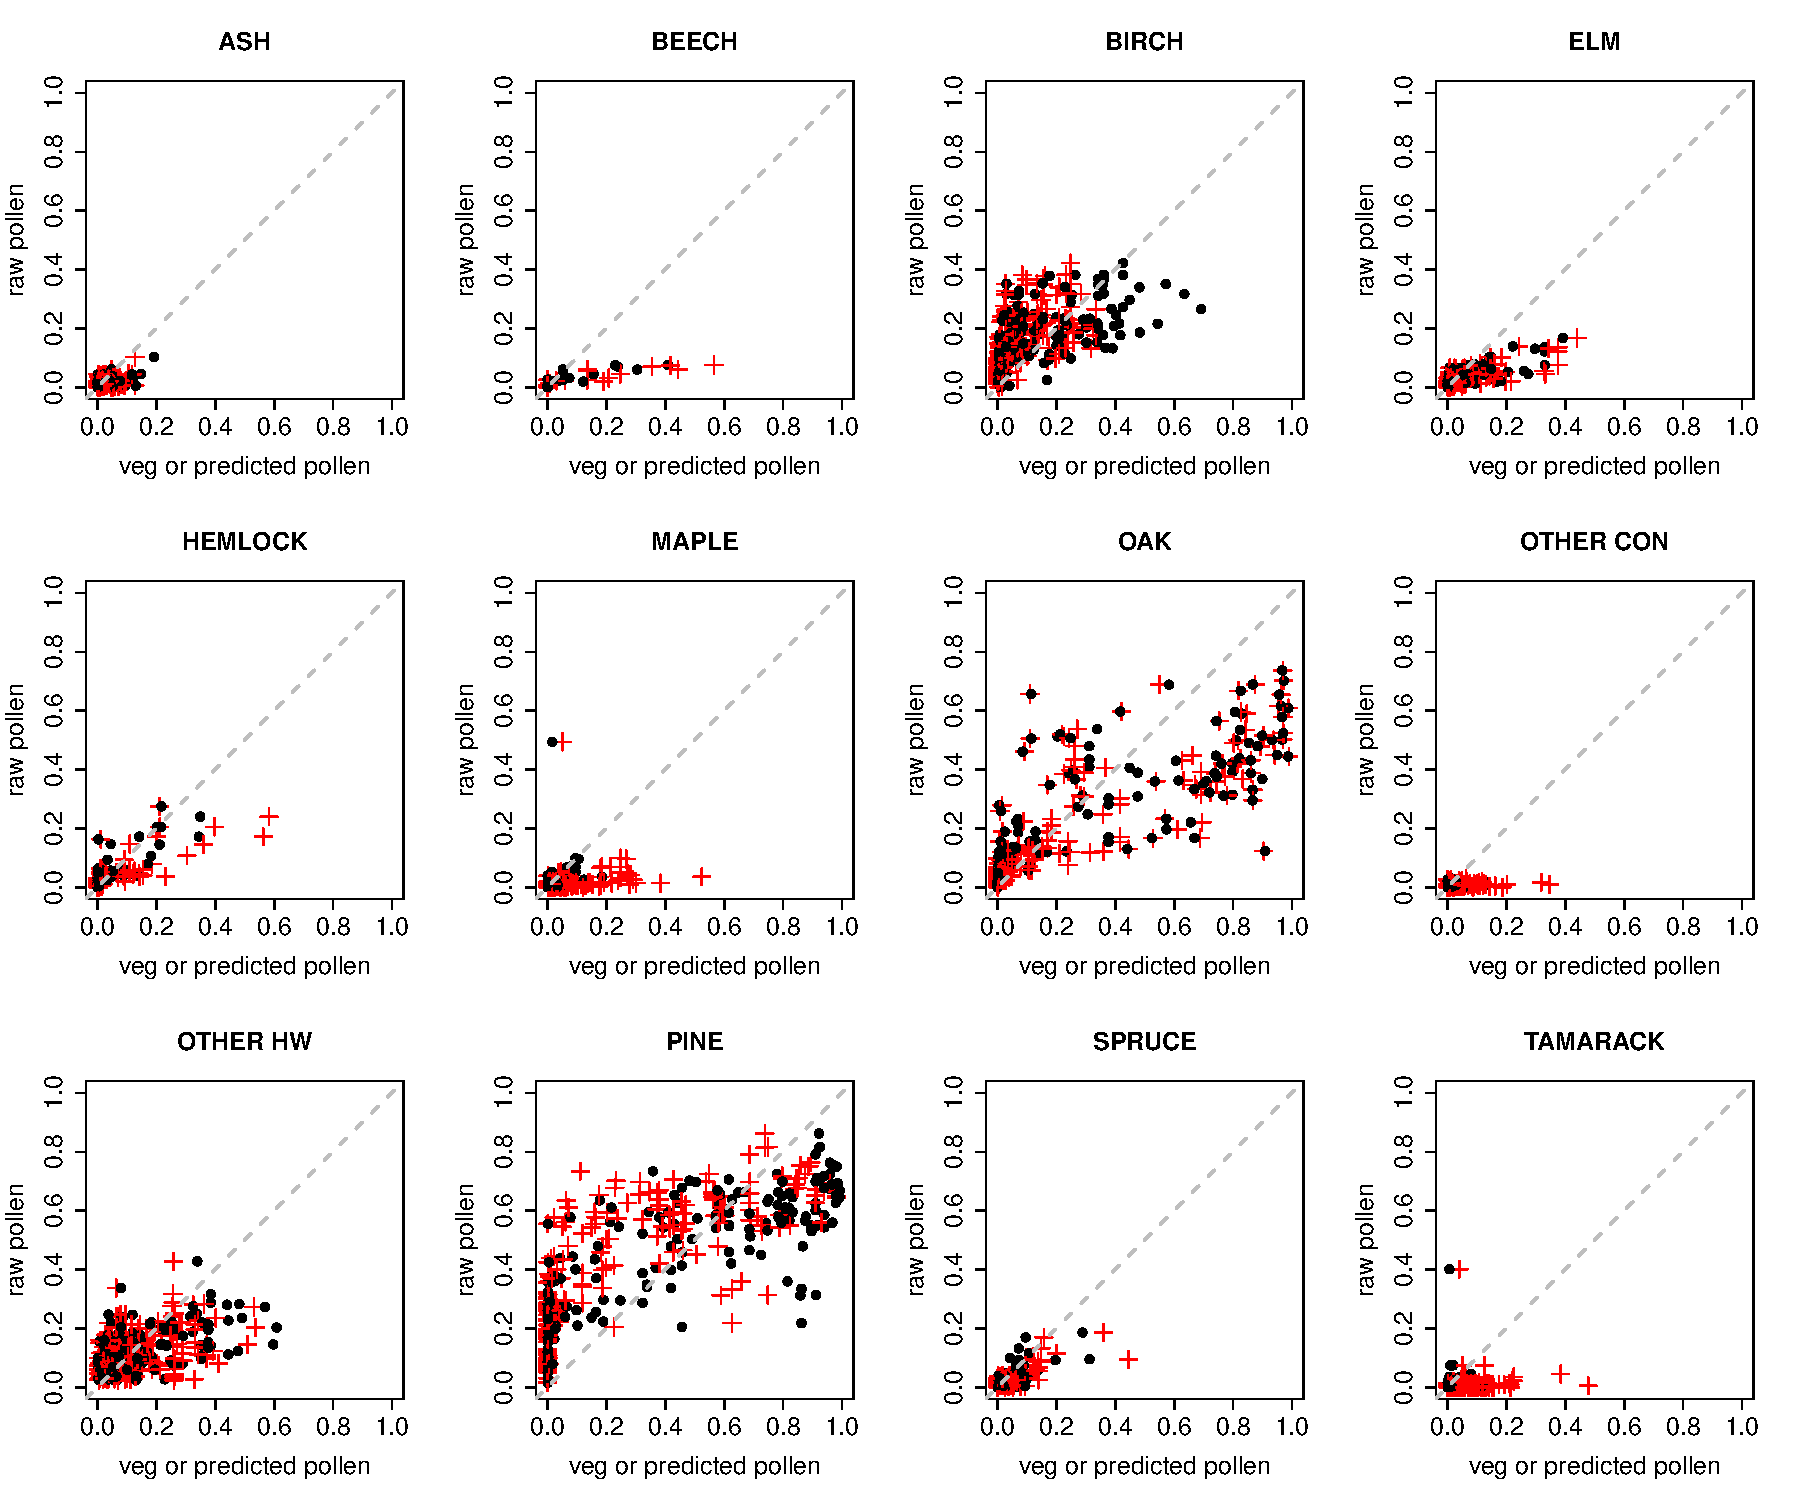
\includegraphics[width=7in]{figures/pollen_focal_scaled.pdf}
% \caption{}
% \label{fig:focal_scaled}
% \end{figure}

%PLS and pollen pie maps
\begin{figure}
\centering
\begin{tabular}{c}
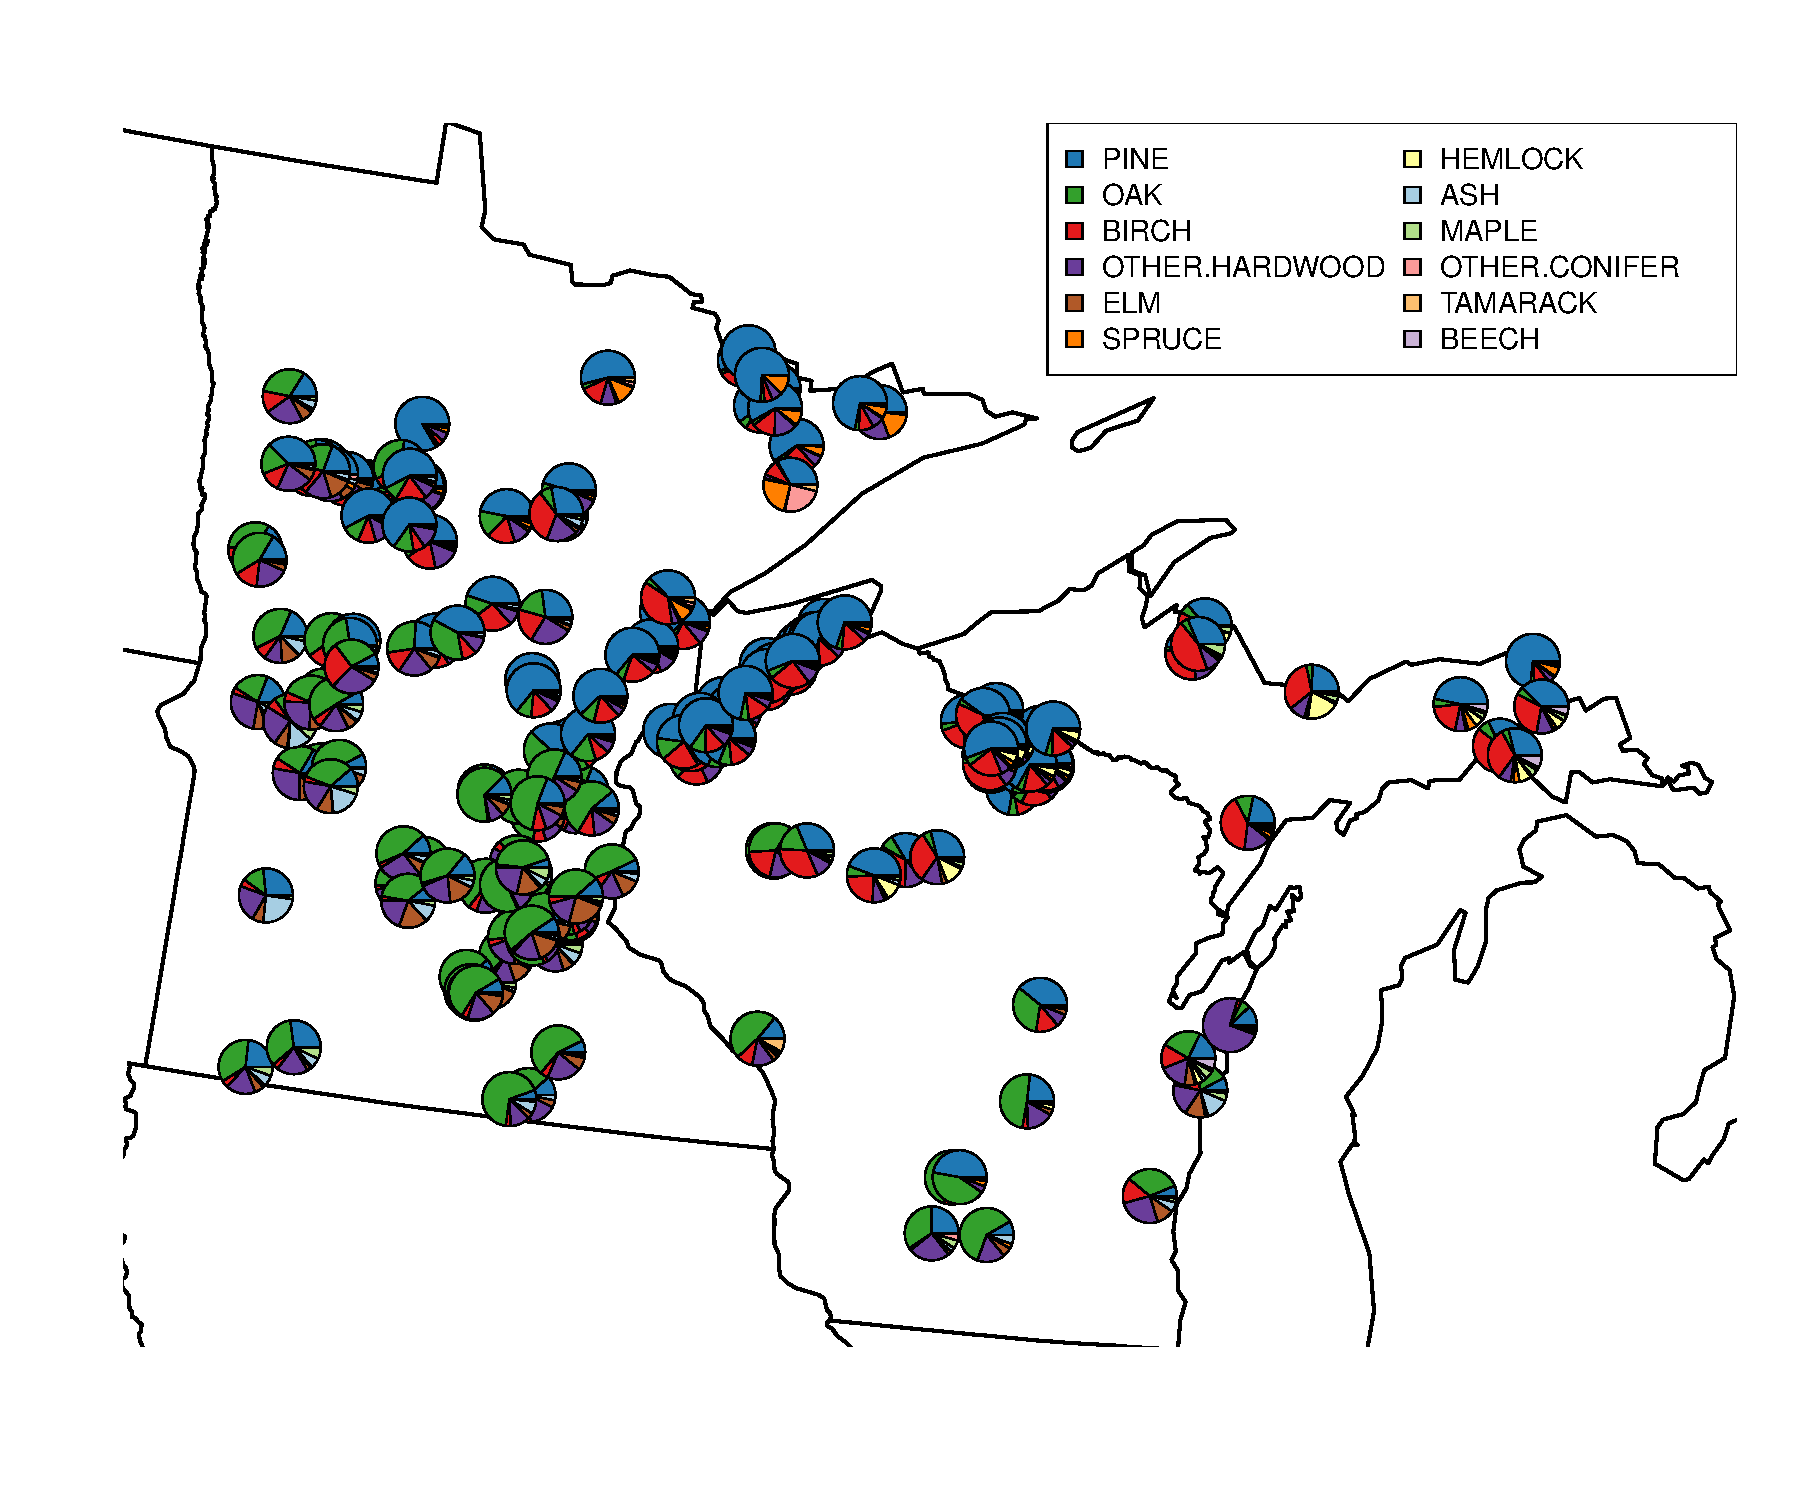
\includegraphics[width=5in]{figures/pie_plot_pollen_UMW_v01.pdf} \\
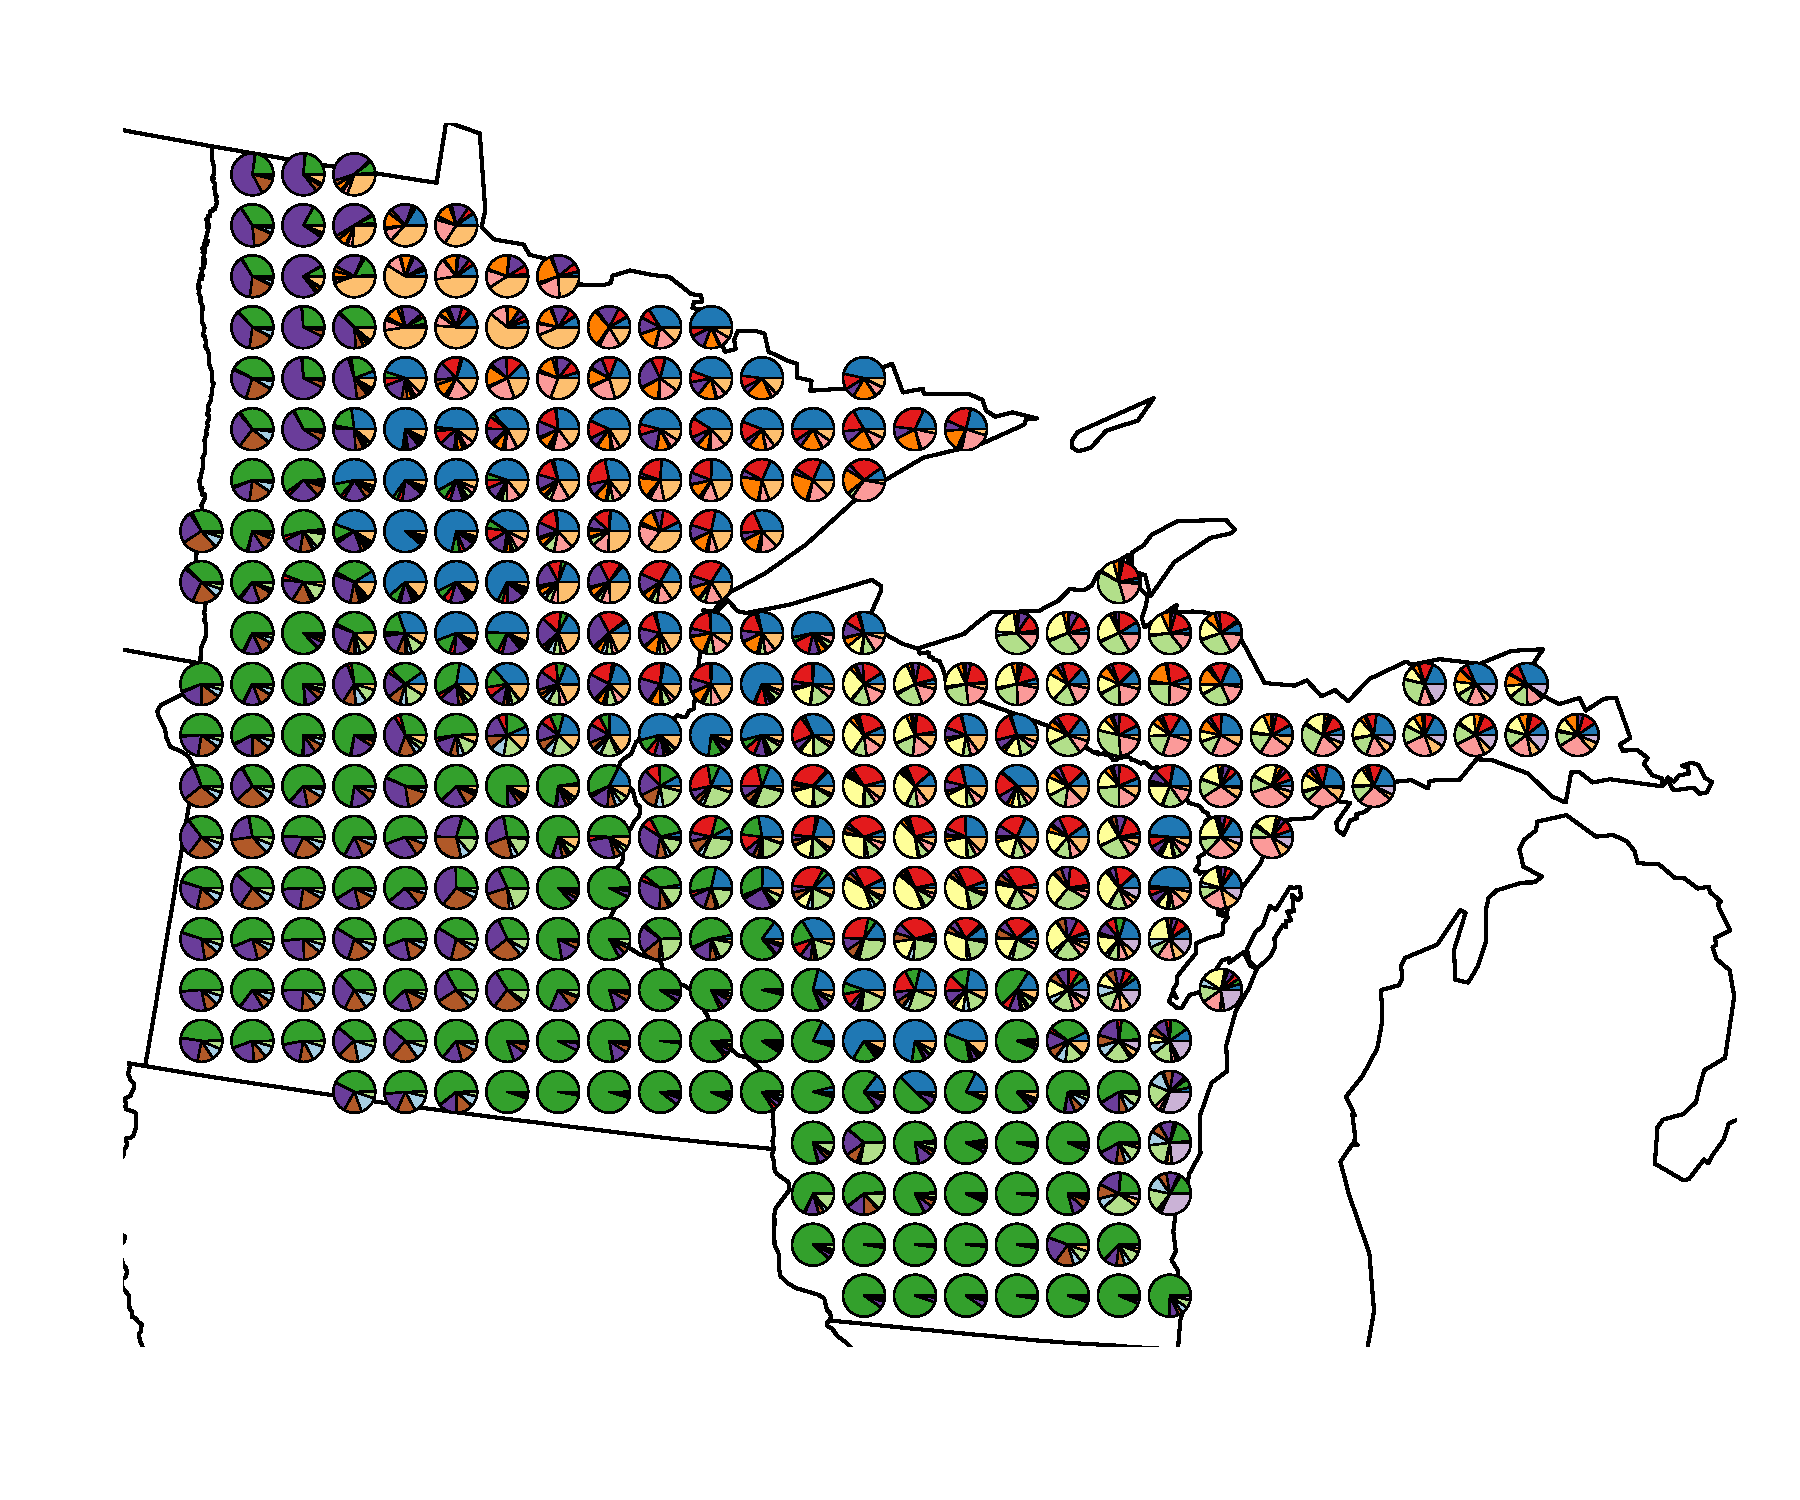
\includegraphics[width=5in]{figures/pie_plot_pls_UMW_v01.pdf}
\end{tabular}
\caption{Pie maps depicting the relative composition of pollen (top)
  and PLS vegetation (bottom) from the data. Note that the PLS data
  has been aggregated to a coarser resolution for illustrative
  purposes.}
\label{fig:pie}
\end{figure}

%veg and pollen heat maps: pine
\begin{figure}
\centering
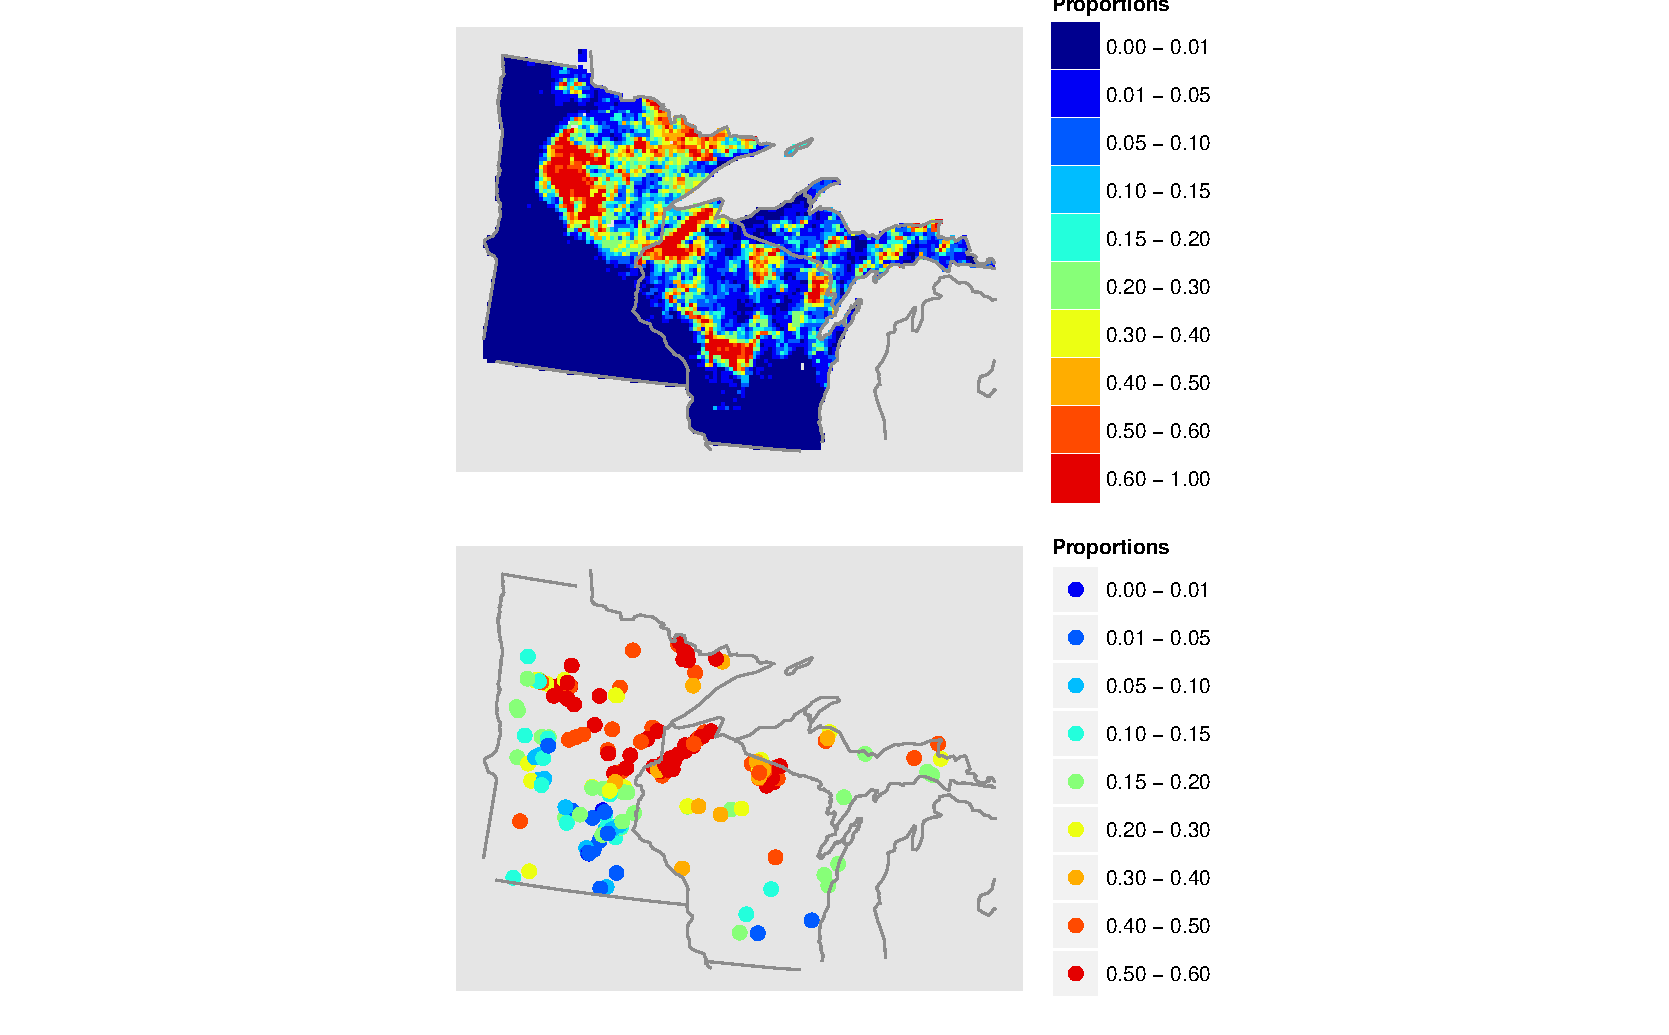
\includegraphics[width=7in]{figures/maps_compare_PINE.pdf}
\caption{Heat maps showing the range limits of Pine in the PLS composition data (top) and the sediment pollen (bottom).}
\label{fig:compare_maps_PINE}
\end{figure}

%veg and pollen heat maps: birch
\begin{figure}
\centering
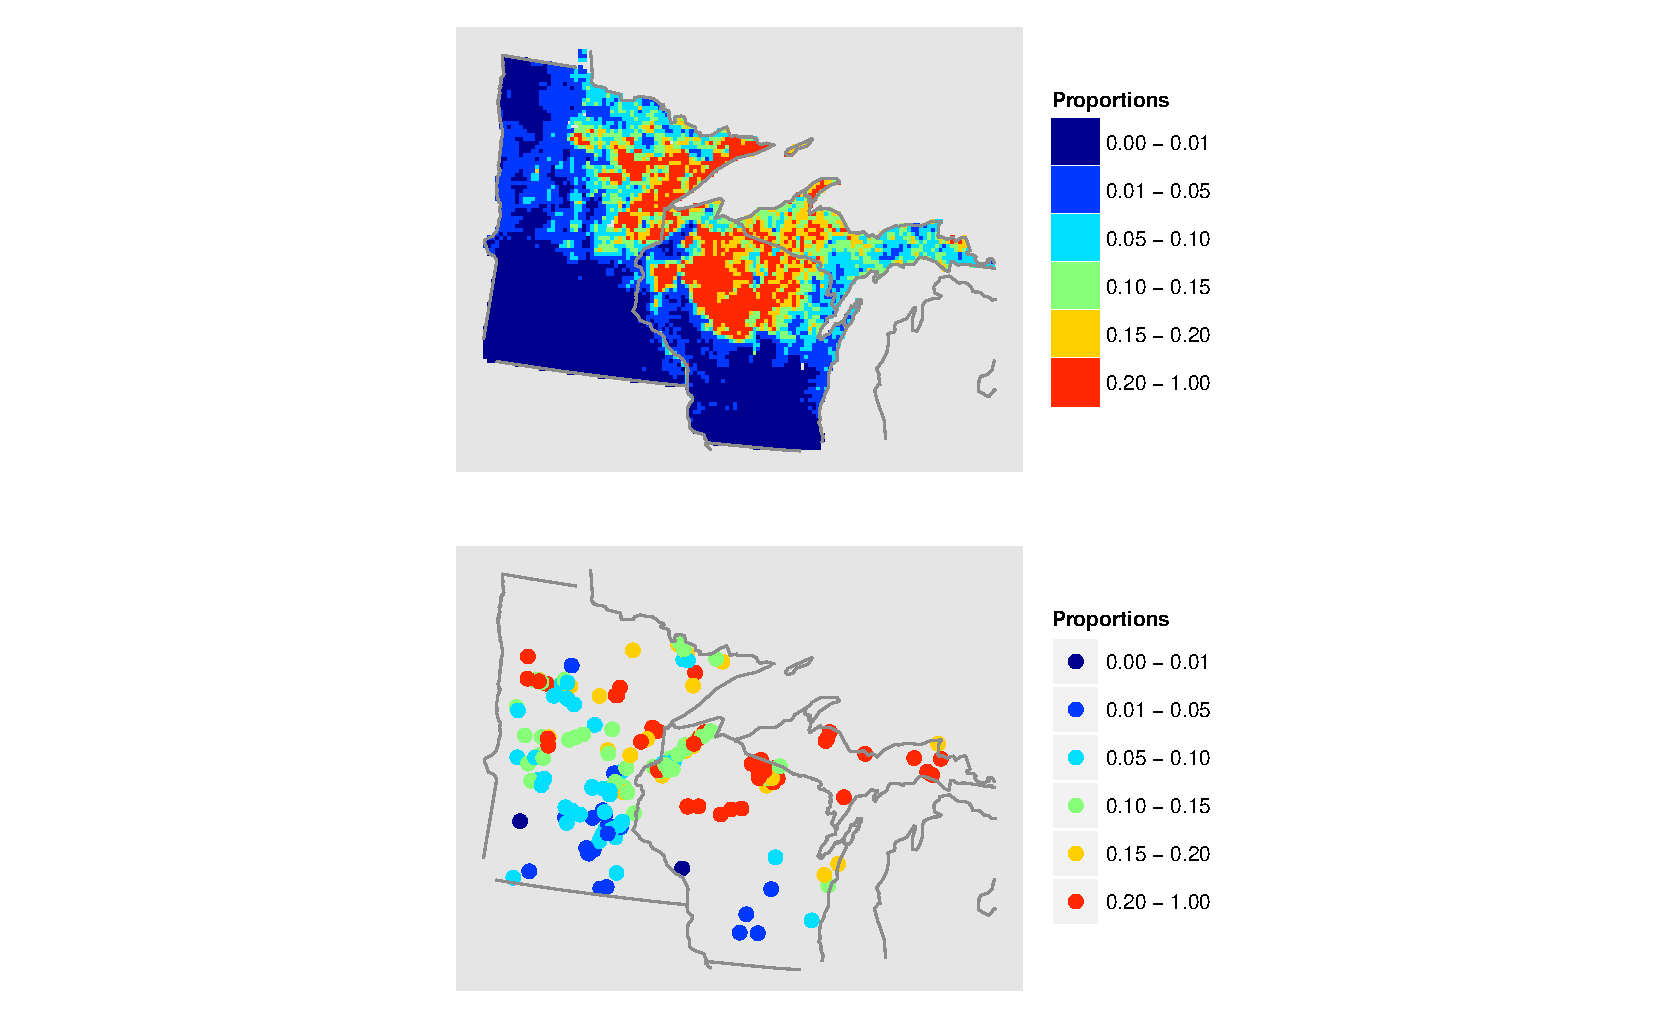
\includegraphics[width=7in]{figures/maps_compare_BIRCH.pdf}
\caption{Heat maps showing the range limits of Birch in the PLS composition data (top) and the sediment pollen (bottom)}
\label{fig:compare_maps_PINE}
\end{figure}

%pollen raw versus scaled focal
\begin{figure}
\centering
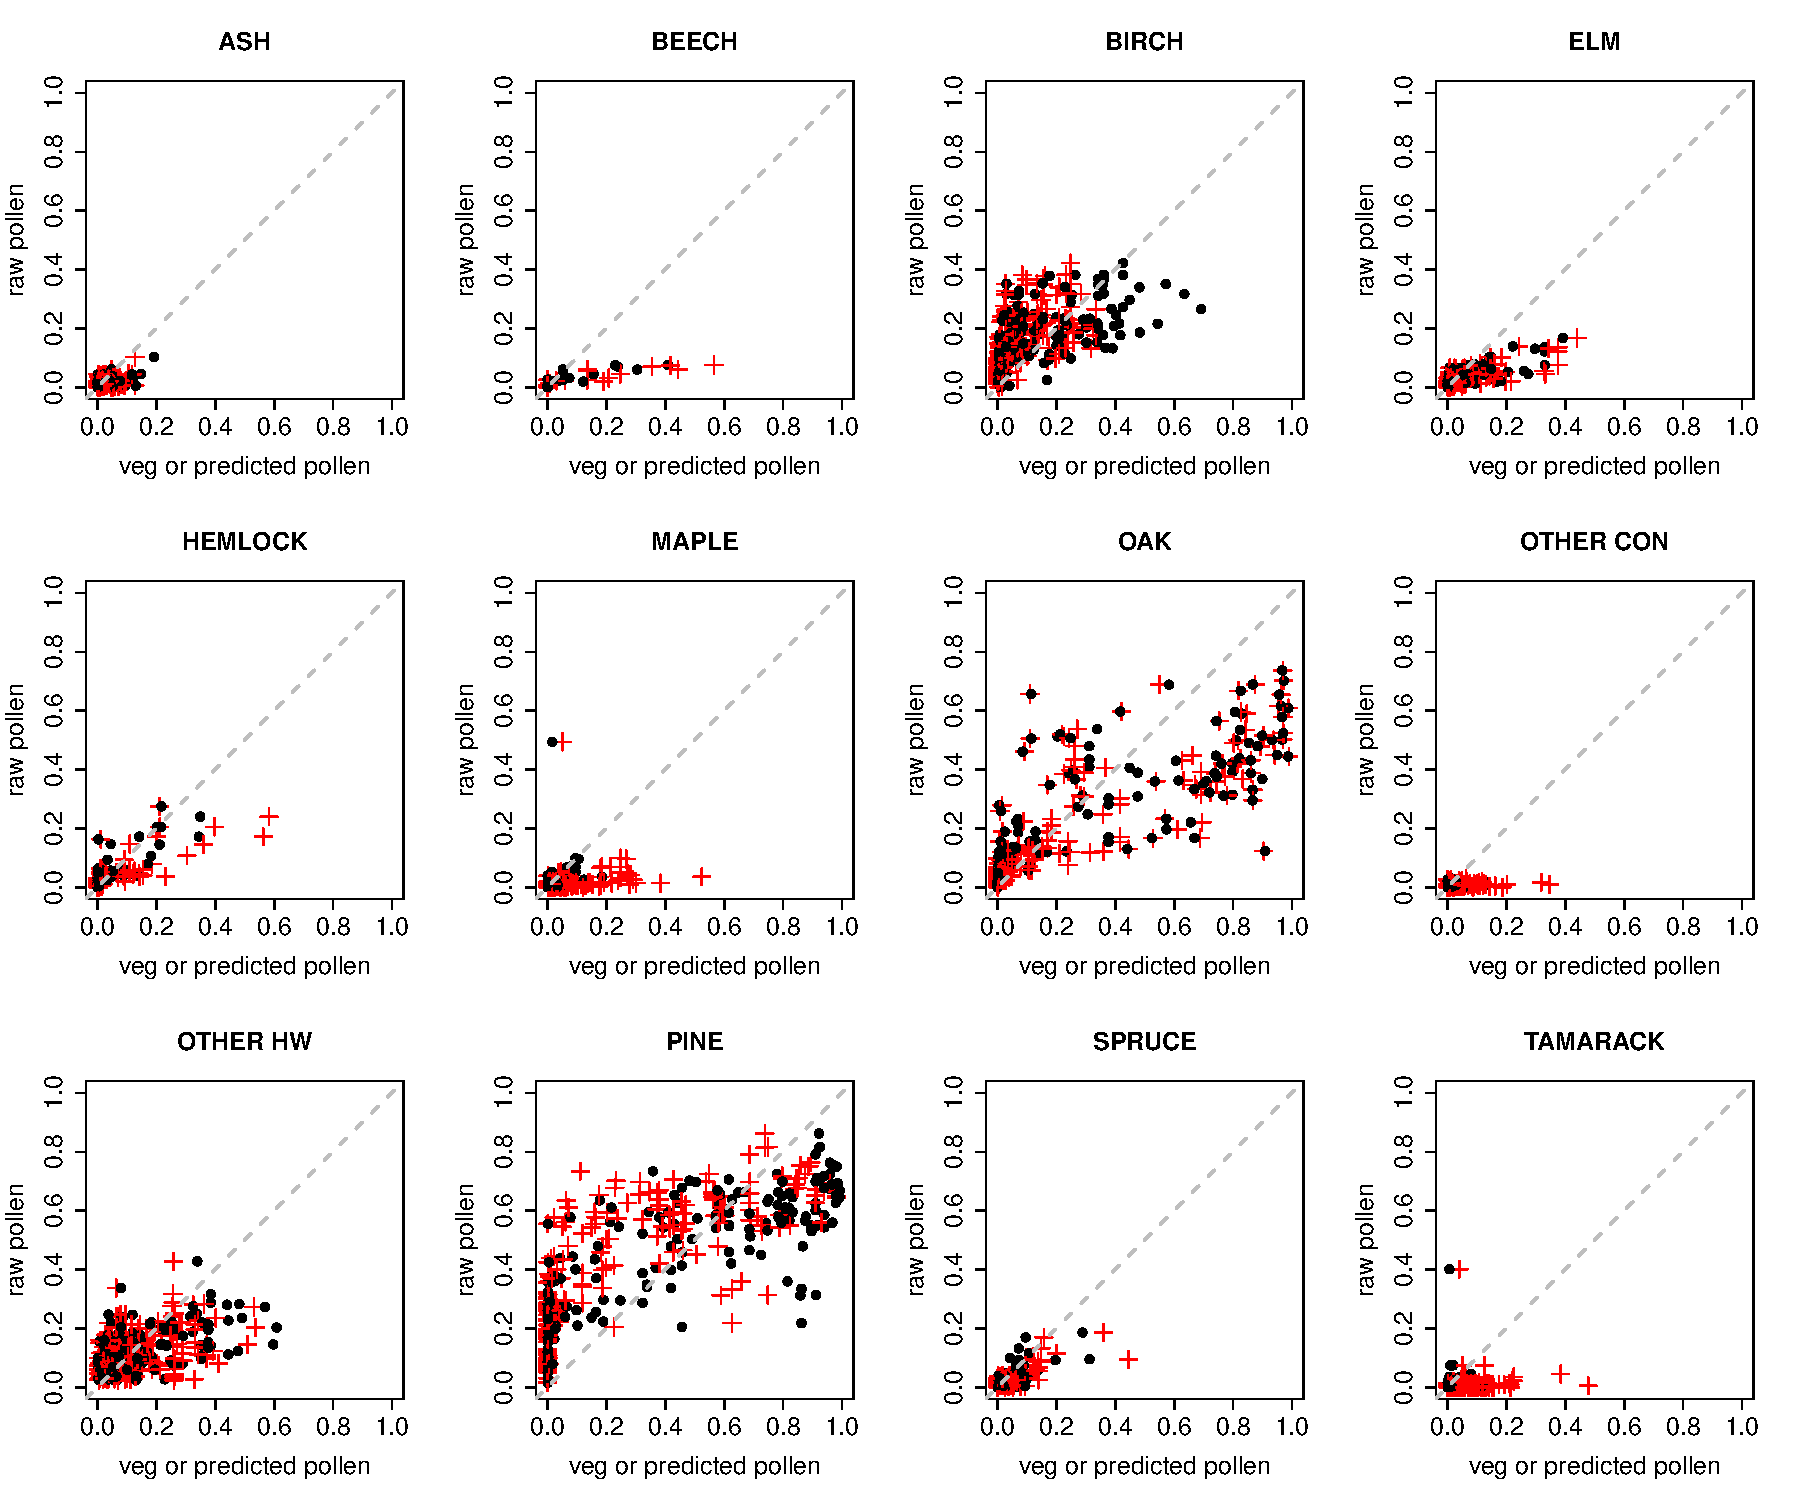
\includegraphics[width=7in]{figures/pollen_focal_scaled.pdf}
\caption{Pollen proportions plotted against local vegetation proportions (red crosses) or local vegetation proportion scaled by $\phi$ (black dots), by taxon.}
\label{fig:focal_scaled}
\end{figure}

%pollen raw versus predicted
\begin{figure}
\centering
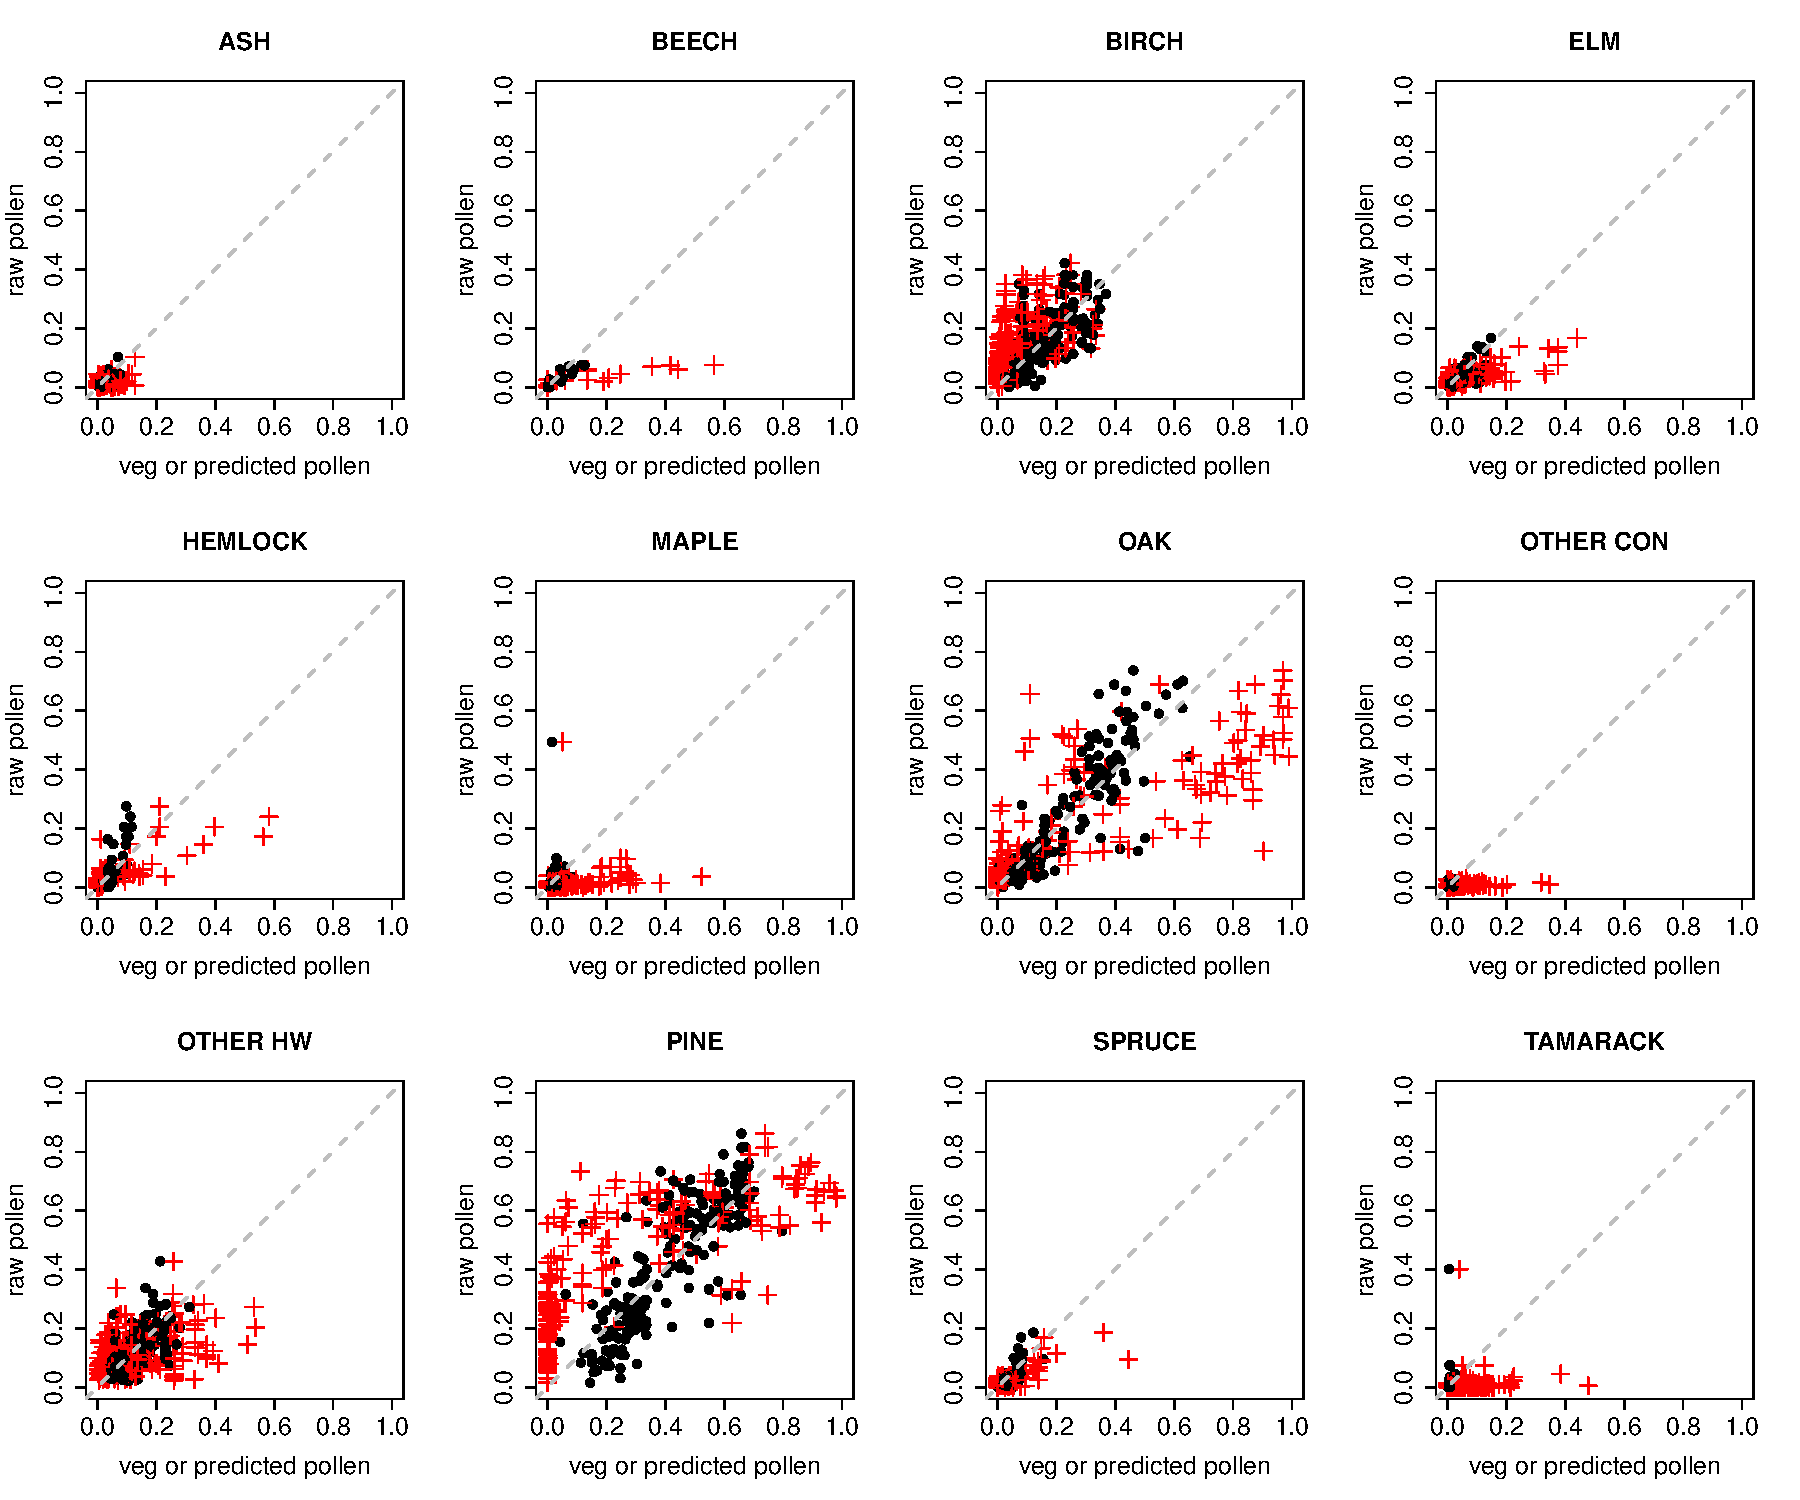
\includegraphics[width=7in]{figures/pollen_preds.pdf}
\caption{Pollen proportions plotted against local vegetation proportions (red crosses) or model-predicted pollen (black dots), by taxon.}
\label{fig:preds}
\end{figure}

%phi (differential production)
\begin{figure}
\centering
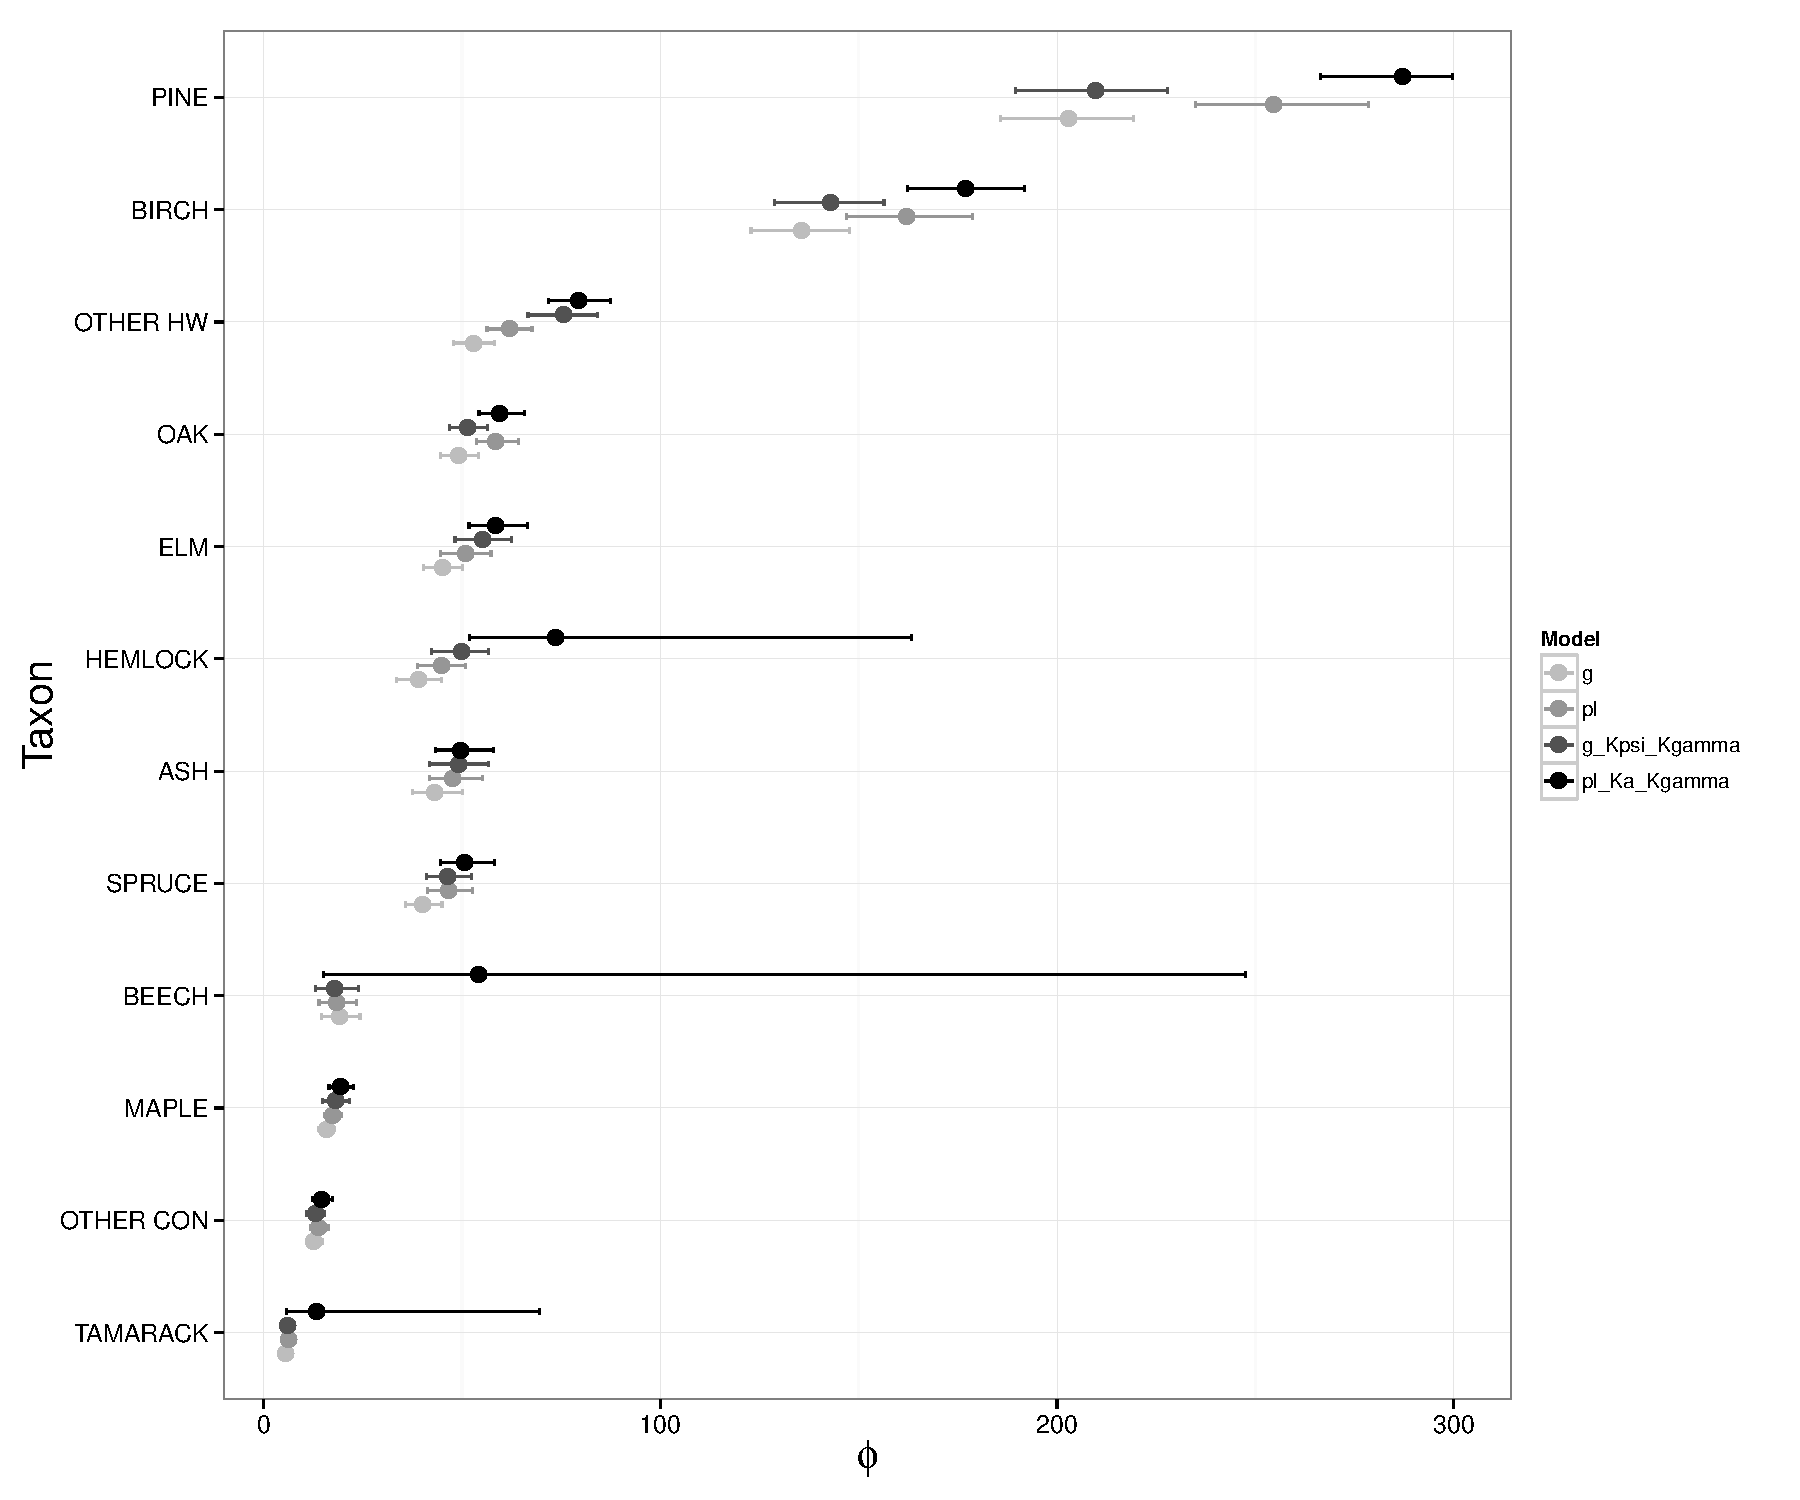
\includegraphics[width=7in]{figures/phi.pdf}
\caption{Mean values and 95\% credible intervals for the estimated values of the differential production parameter $\phi$.}
\label{fig:phi}
\end{figure}

%proportion pollen versus radius
\begin{figure}
\centering
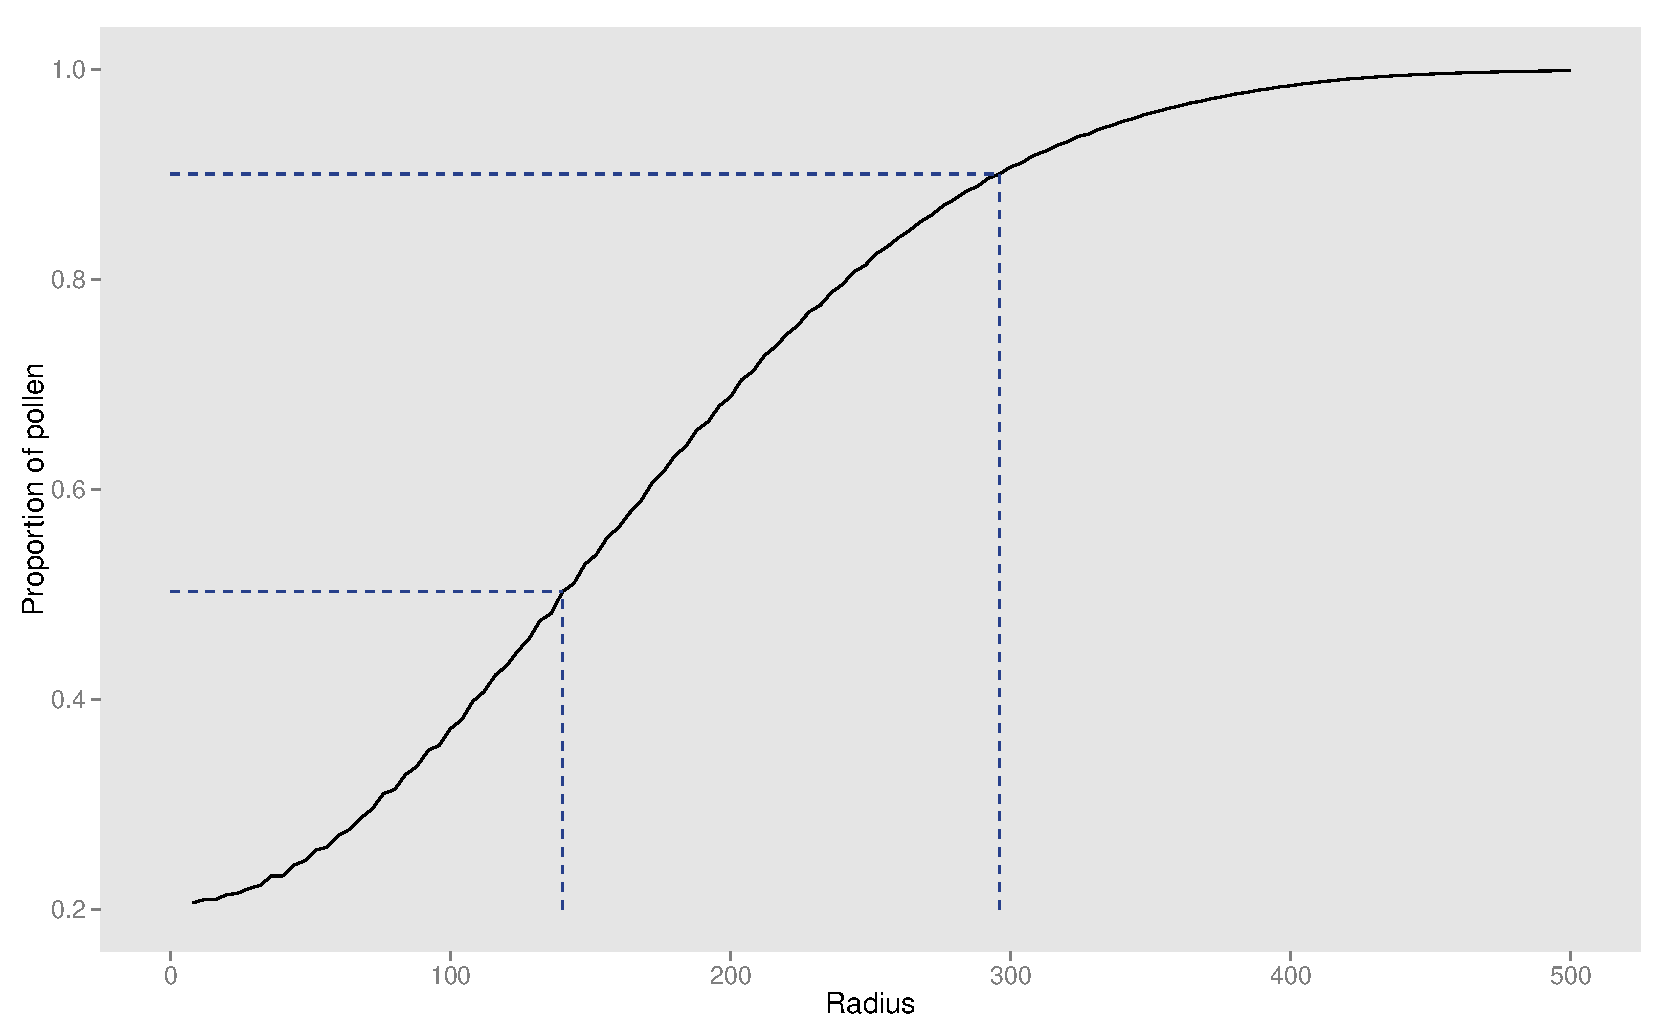
\includegraphics[width=7in]{figures/dispersal_vs_distance.pdf}
\caption{Here we consider pollen produced by a focal cell, and plot the proportion of deposited pollen as a function of the radius of a circle centered at the focal cell.}
\label{fig:dvd}
\end{figure}

%psi: vary psi case
\begin{figure}
\centering
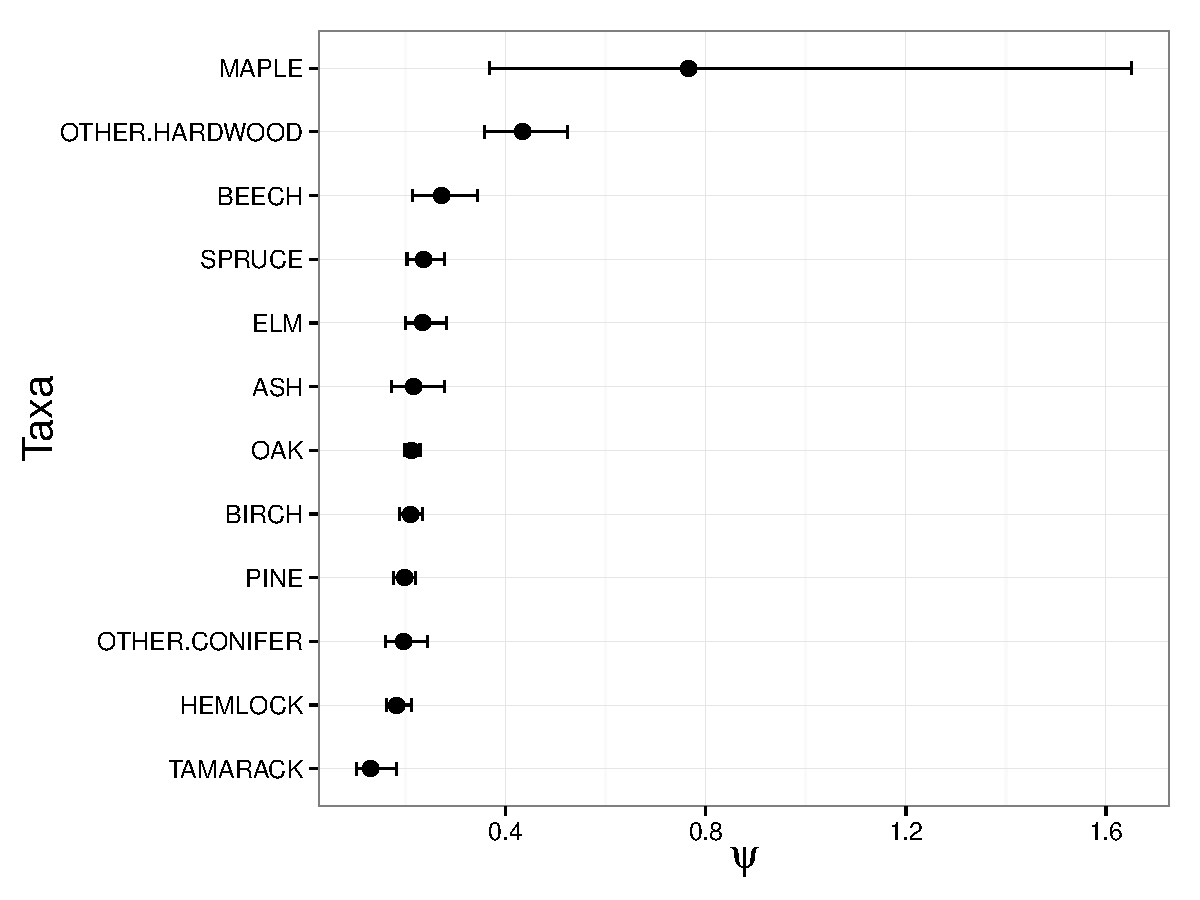
\includegraphics[width=7in]{figures/psi_vary_psi.pdf}
\caption{Mean values of 95\% credible intervals for the estimated values of the dispersal kernel spread $\psi$ for the case where we let $\psi$ vary by taxon.}
\label{fig:psi_vary_psi}
\end{figure}

%phi: vary phi case
\begin{figure}
\centering
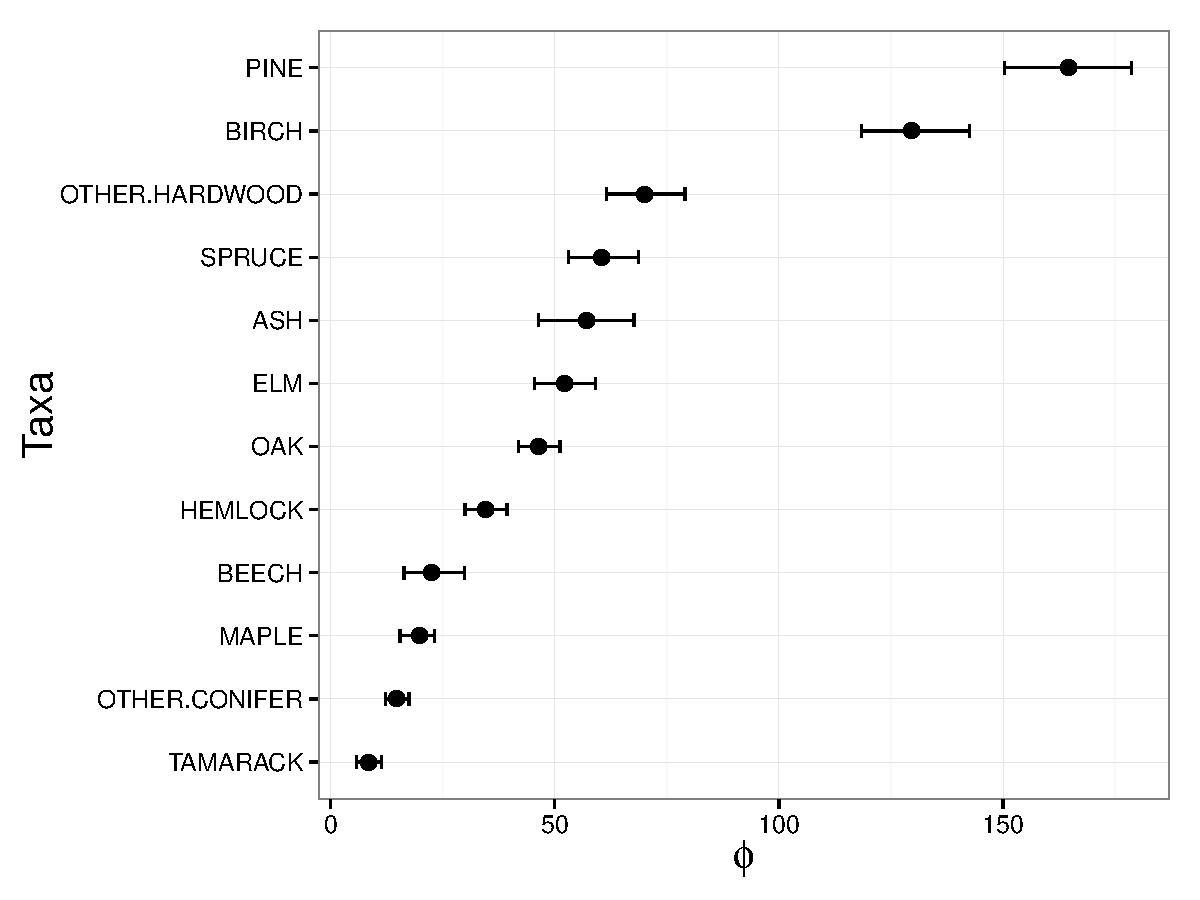
\includegraphics[width=7in]{figures/phi_vary_psi.pdf}
\caption{Mean values of 95\% credible intervals for the estimated values of the differential production parameter $\phi$ for the case where $\psi$ varied by taxon.}
\label{fig:phi_vary_psi}
\end{figure}

%potential pollen maps by taxon
\begin{figure}
\centering
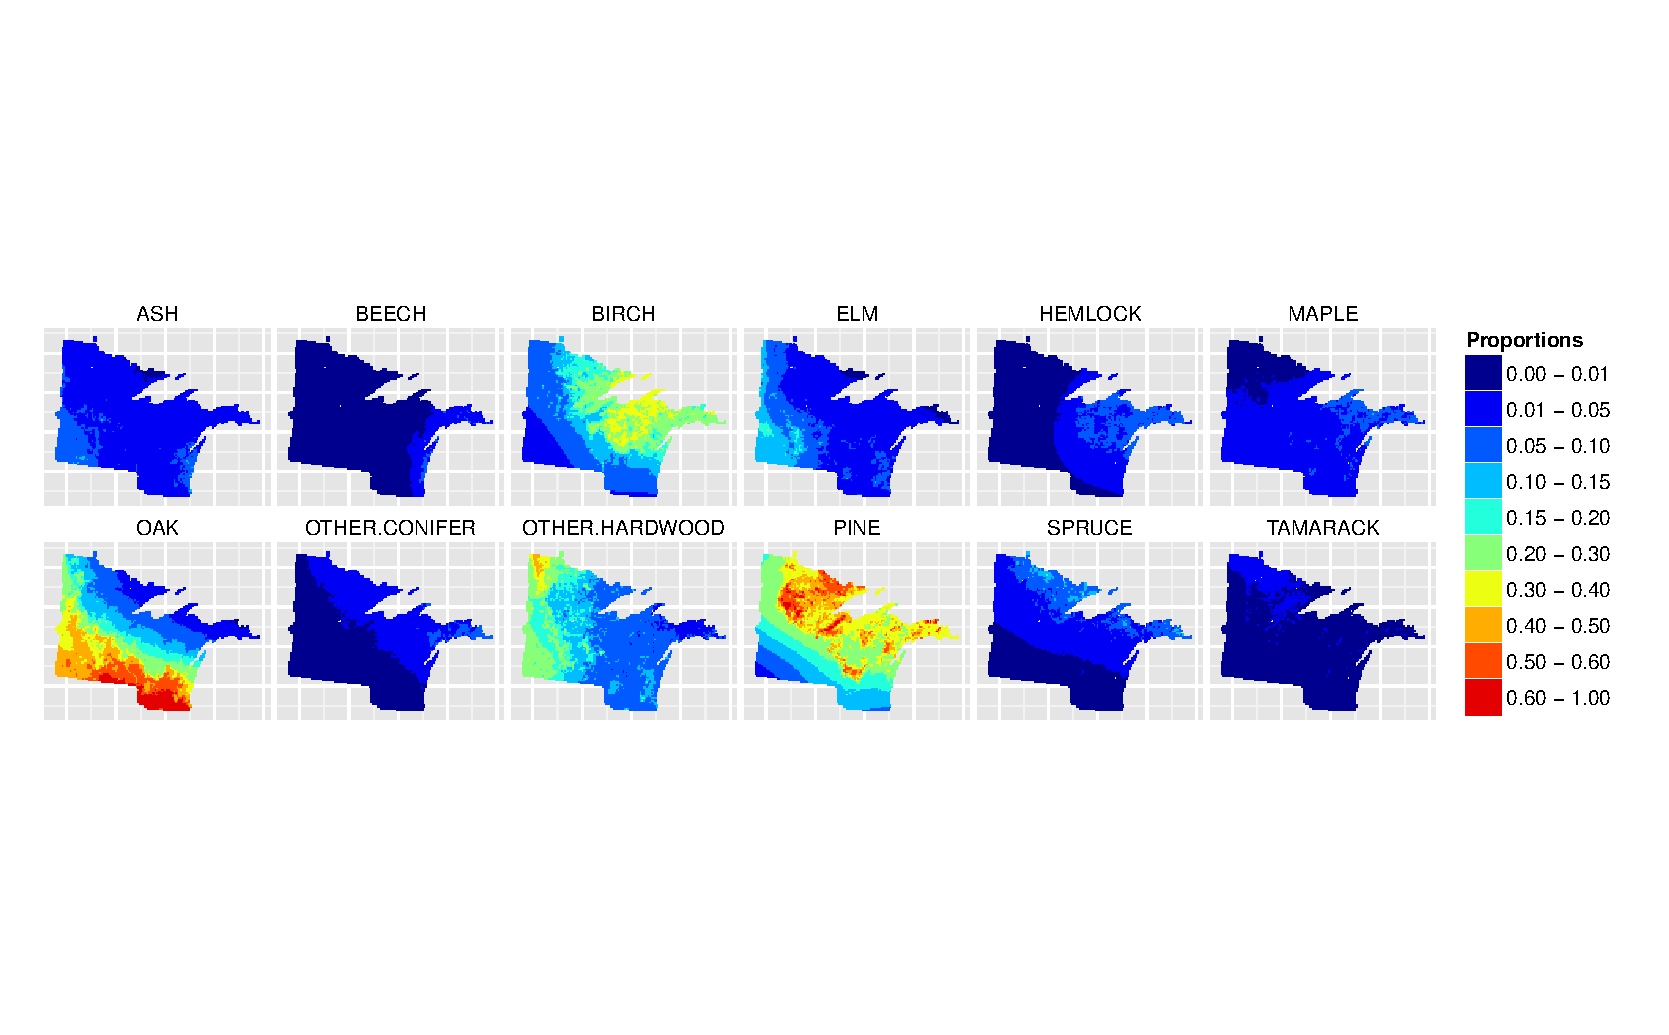
\includegraphics[width=7in]{figures/maps_pollen.pdf}
\caption{Heat maps of model-predicted pollen for each grid cell in the domain, by taxon.}
\label{fig:maps_pollen}
\end{figure}

%PLS data maps by taxon
\begin{figure}
\centering
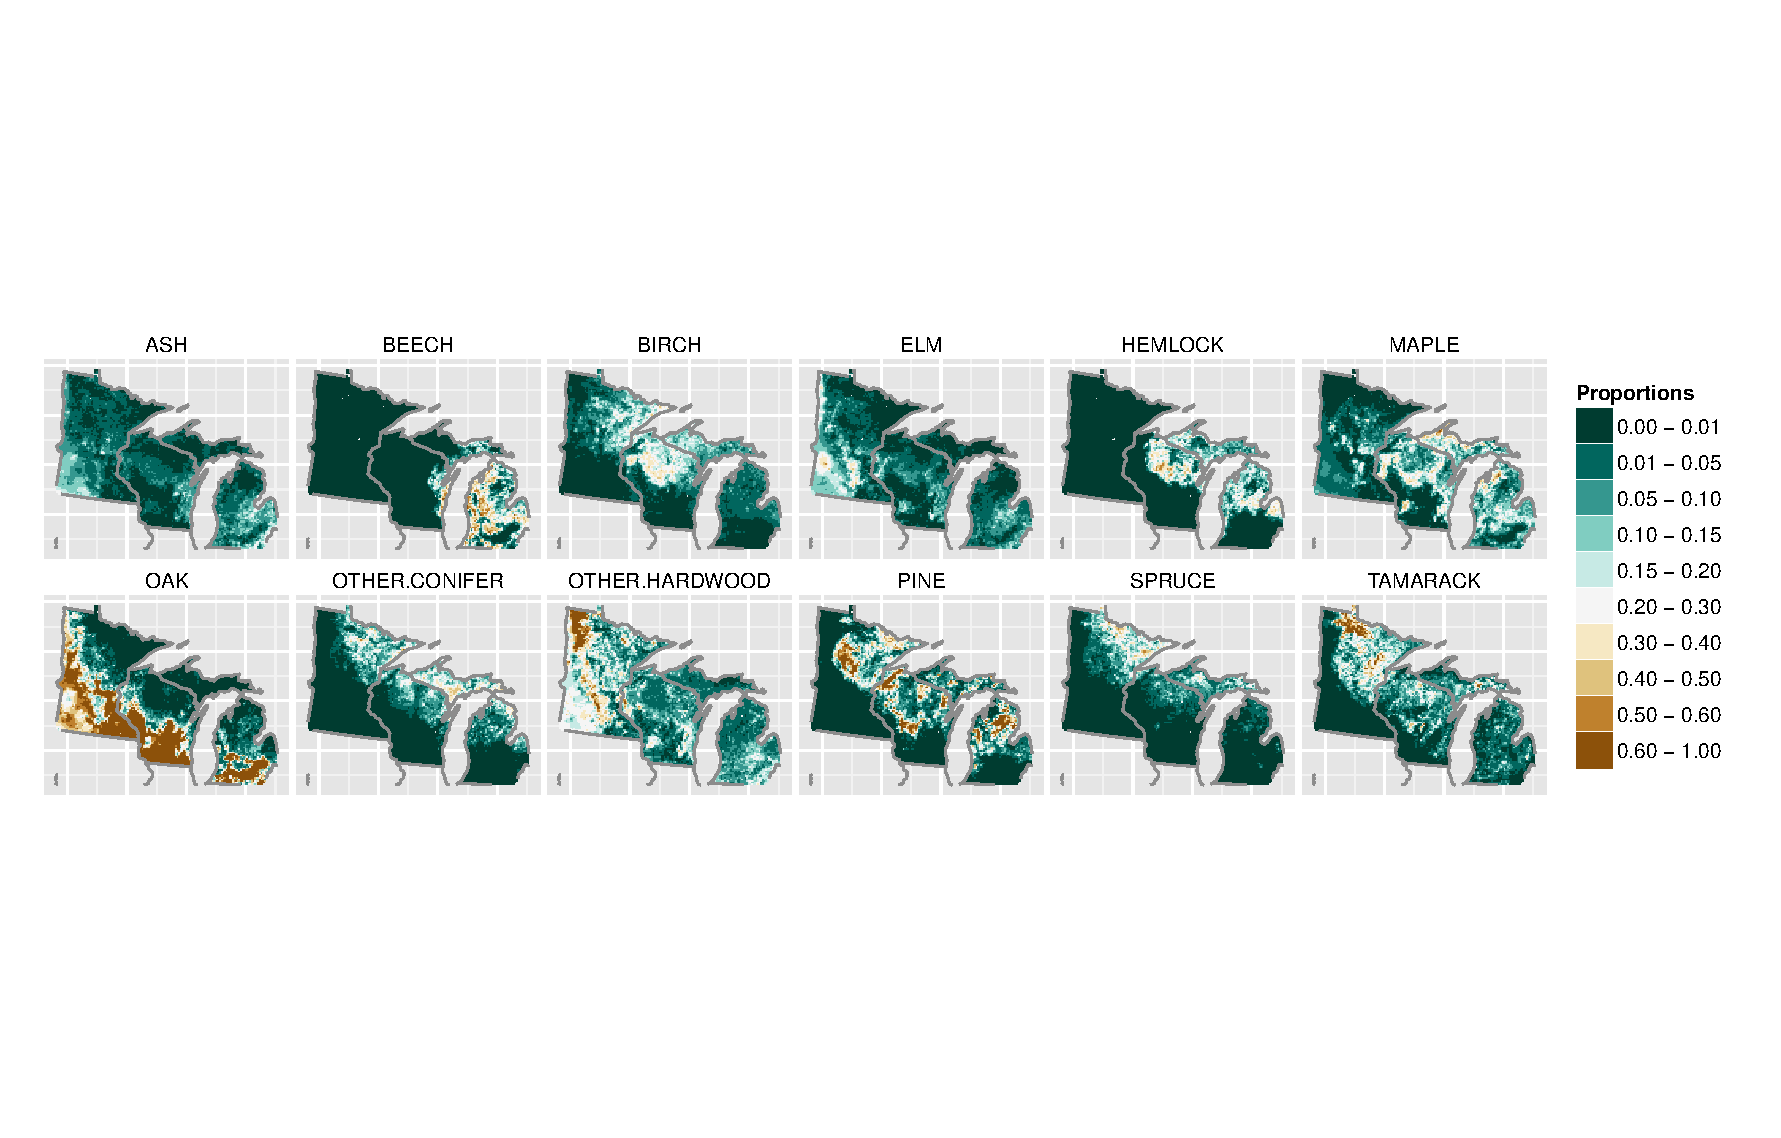
\includegraphics[width=7in]{figures/maps_veg.pdf}
\caption{Heat maps of the PLS data, by taxon.}
\label{fig:maps_pollen}
\end{figure}





